\section{Định hướng: bài báo giải quyết điều gì?}
\label{sec:orientation}

Hãy tưởng tượng bạn phụ trách chiến dịch cho một mẫu điện thoại mới. Bạn có lượng tìm kiếm
theo tuần của vài từ khóa tại nhiều quốc gia. Ba câu hỏi tự nhiên xuất hiện:

\begin{enumerate}
  \item \textbf{Ở đâu?} Quốc gia nào đang quan tâm nhiều đến từng sản phẩm?
  \item \textbf{Lan từ đâu sang đâu?} Mức quan tâm tăng ở Mỹ rồi vài tuần sau tăng ở Việt Nam
        có phải là một dấu hiệu lan truyền?
  \item \textbf{Tiếp theo sẽ thế nào?} Tuần tới, tháng tới, lượng tìm kiếm ở mỗi nơi ra sao?
\end{enumerate}

D-Tracker được thiết kế để trả lời đồng thời ba câu hỏi này trên một \emph{luồng tensor}
(tensor stream) chứ không chỉ trên một bảng thời gian đơn giản. Điểm cốt lõi không phải là
dự báo bằng một mạng nơ-ron lớn, mà là xây một mô hình nhỏ, có ý nghĩa vật lý, vừa nén dữ liệu
vừa giải thích được các kiểu thay đổi.

\begin{keypoint}
D-Tracker tách dữ liệu quan sát thành \textbf{trend + seasonal + outlier}. Phần trend được nén
thành một lõi nhỏ; lõi này tiến hóa theo một hệ \textbf{reaction--diffusion} để biểu diễn tăng
trưởng và lan truyền giữa các nhóm địa điểm. Mô hình được cập nhật khi dữ liệu mới đến và tự
chuyển sang mô hình mới khi cấu trúc thay đổi.
\end{keypoint}

\subsection{Một ví dụ nhỏ để thấy ba loại tín hiệu}

Bảng~\ref{tab:running-example} là dữ liệu \textbf{minh họa do tài liệu này tạo}, không phải kết
quả của paper. Mỗi ô là chỉ số quan tâm từ 0 đến 100.

\begin{table}[htbp]
  \centering
  \small
  \caption{Ví dụ minh họa: cùng một từ khóa, mức quan tâm khác nhau theo địa điểm và thời gian.}
  \label{tab:running-example}
  \begin{tabular}{llrrr}
    \toprule
    Từ khóa & Địa điểm & Tuần 1 & Tuần 2 & Tuần 3 \\
    \midrule
    iPhone & Hoa Kỳ & 80 & 84 & 90 \\
    iPhone & Việt Nam & 15 & 22 & 35 \\
    Galaxy & Hoa Kỳ & 45 & 40 & 32 \\
    Galaxy & Việt Nam & 30 & 34 & 40 \\
    \bottomrule
  \end{tabular}
\end{table}

Có ít nhất ba điều đang diễn ra. Thứ nhất, ``iPhone'' tăng ở cả hai nơi, nhưng mạnh hơn ở Hoa Kỳ.
Thứ hai, mức tăng ở Việt Nam xuất hiện sau Hoa Kỳ trong ví dụ này --- một \emph{ứng viên} của
lan truyền quan tâm, chưa phải bằng chứng nhân quả. Thứ ba, ``Galaxy'' đi xuống ở Hoa Kỳ nhưng
đi lên ở Việt Nam, nên xu hướng không giống nhau cho mọi cặp từ khóa--địa điểm. Dữ liệu thật
còn có mùa vụ (ra mắt sản phẩm, khuyến mãi cuối năm) và những cú tăng bất thường.

\begin{plainwords}
Nếu chỉ nhìn một đường, ta dễ nhầm mùa vụ với xu hướng và nhầm một lần tăng đột biến với lan
truyền. D-Tracker tách ba nguồn tín hiệu trước, rồi mới tìm quy luật trong phần xu hướng.
\end{plainwords}

\subsection{Ba thách thức và ba lời hứa}

Paper nhấn mạnh ba khó khăn. Dữ liệu có \textbf{pattern phức tạp} (trend, mùa vụ, lan truyền,
outlier); các pattern \textbf{thay đổi theo thời gian}; và dữ liệu là tensor nhiều chiều,
gần như \textbf{bán vô hạn} theo thời gian. Ba tính chất mà tác giả dùng để tóm tắt giải pháp
được nêu trong phần mở đầu và kết luận:

\begin{description}[leftmargin=1.8em,style=nextline]
  \item[Interpretable --- diễn giải được.] Lõi động học và các hệ số không âm cho biết nhóm
  địa điểm/từ khóa nào liên quan đến dynamics nào, và dòng lan truyền đi theo hướng nào.
  Đây là diễn giải \emph{theo cấu trúc mô hình}, không phải chứng minh quan hệ nhân quả.
  \item[Automatic --- tự động.] Số chiều ẩn và thời điểm đổi mô hình được chọn bằng một tiêu
  chuẩn nén dữ liệu (MDL), thay vì người dùng thử từng cấu hình. Vẫn có các tham số của bộ tối ưu,
  nhưng không phải chọn tay ``hai nhóm hay ba nhóm?'' cho từng giai đoạn.
  \item[Scalable --- mở rộng được.] Mỗi lần chỉ xử lý một cửa sổ gần nhất có độ dài cố định,
  nên thời gian xử lý không tăng theo tổng chiều dài của toàn bộ stream. Paper báo cáo nhanh hơn
  đối thủ tới 8.0 lần và ``cải thiện tới 57\%''; câu nói về 57\% không nêu metric hay mẫu số, nên
  đây chỉ là con số paper công bố, không phải kết quả tái hiện hay một effect size đã chuẩn hóa
  trong repo này.
\end{description}

\begin{commonmistake}
``Scalable'' ở đây không có nghĩa mọi phép tính là $O(1)$. Nó có nghĩa chi phí xử lý một bước
stream không phụ thuộc vào việc stream đã dài bao nhiêu, vì ta chỉ giữ một cửa sổ. Chi phí vẫn
tăng theo số từ khóa, số địa điểm và số chiều ẩn.
\end{commonmistake}

\subsection{Nhìn thấy kết quả trước khi học cơ chế}

\begin{figure}[htbp]
  \centering
  \begin{subfigure}[t]{0.92\linewidth}
    \centering
    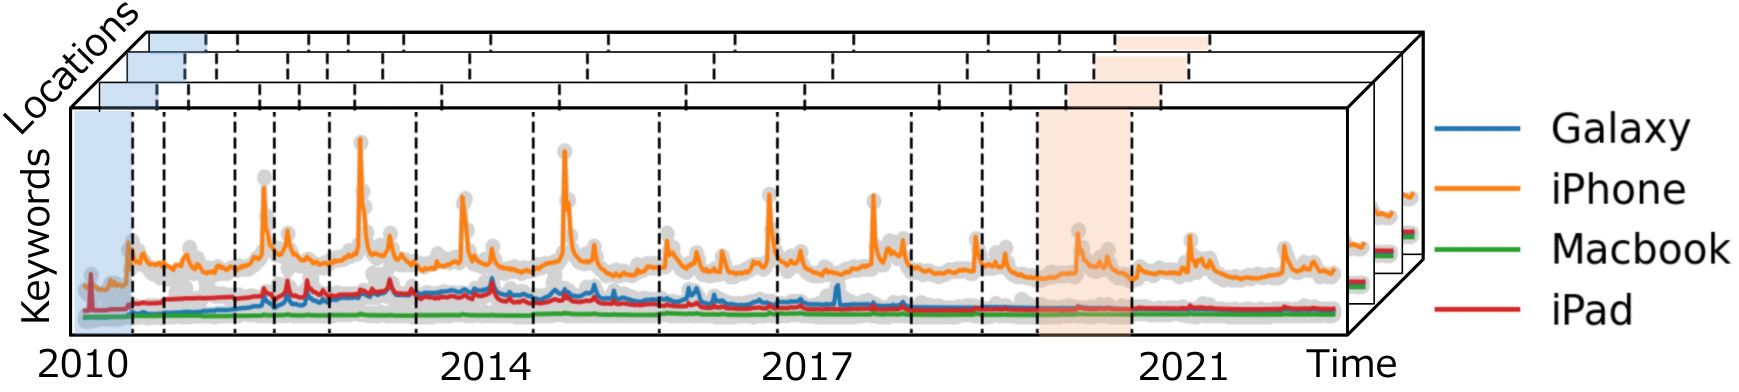
\includegraphics[width=\linewidth]{figures/Figure1_a.png}
    \caption{Dữ liệu thật (xám) và mô hình khớp (màu); các đường chấm dọc đánh dấu lúc đổi mô hình.}
  \end{subfigure}

  \vspace{4mm}
  \begin{subfigure}[t]{0.82\linewidth}
    \centering
    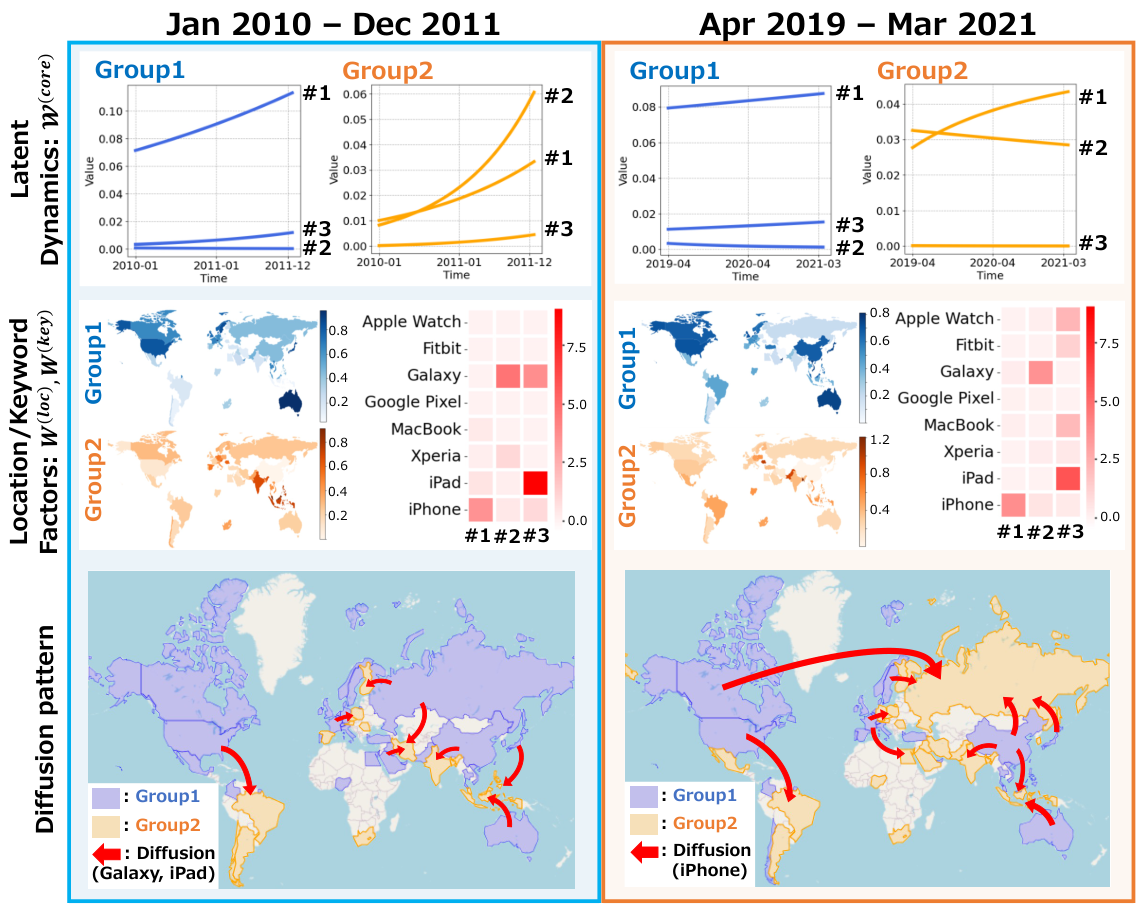
\includegraphics[width=\linewidth]{figures/Figure1_b.png}
    \caption{Lõi dynamics, hệ số địa điểm/từ khóa và bản đồ lan truyền ở hai giai đoạn.}
  \end{subfigure}
  \caption{Sức mạnh mô hình hóa của D-Tracker trên dữ liệu thiết bị. Nguồn: Higashiguchi et al.
  (2025), arXiv:2505.00242v1, Figure~1; hình của tác giả, CC BY 4.0.}
  \label{fig:preview}
\end{figure}

Ở Hình~\ref{fig:preview}(a), mô hình không dùng một bộ tham số cho toàn bộ giai đoạn hiển thị. Các đường
chấm cho thấy nó chia stream thành nhiều giai đoạn và dùng một mô hình cho mỗi giai đoạn. Đây là
cơ chế \emph{regime switching}. Ở Hình~\ref{fig:preview}(b), mỗi cột là một dynamics: đường
trên cùng là lõi $\mathcal{W}^{(\mathrm{core})}$ theo thời gian; hàng giữa là mức liên hệ của
dynamics với các từ khóa và nhóm địa điểm; hàng dưới là mũi tên lan truyền giữa các nhóm. Nhờ
vậy, ta không chỉ có một con số dự báo mà còn có một câu chuyện có thể kiểm tra: dynamics nào,
từ khóa nào, khu vực nào, lan theo hướng nào.

\begin{figure}[htbp]
  \centering
  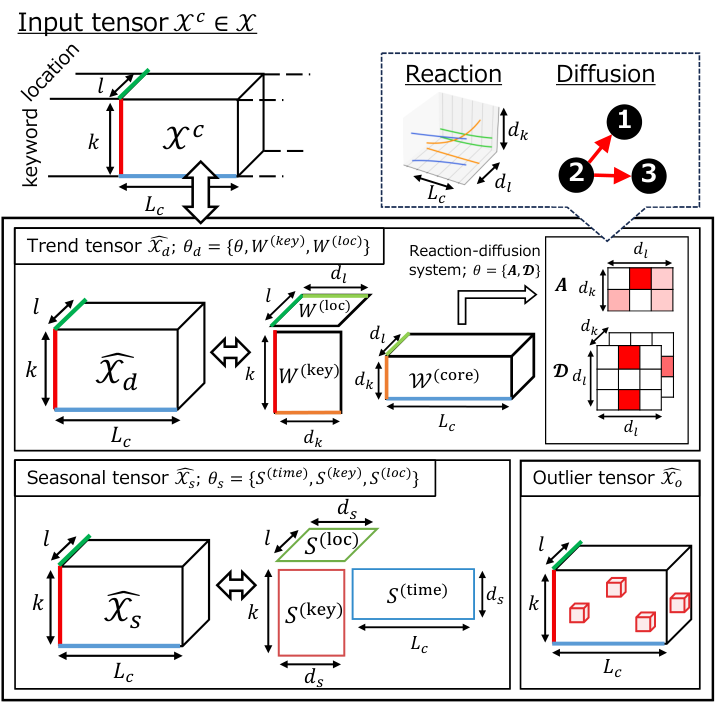
\includegraphics[width=0.72\linewidth]{figures/overview.png}
  \caption{Tổng quan D-Tracker: tensor hiện tại xấp xỉ bằng trend + seasonal + outlier. Nguồn:
  Higashiguchi et al. (2025), arXiv:2505.00242v1, Figure~2; hình của tác giả, CC BY 4.0.}
  \label{fig:overview}
\end{figure}

Hình~\ref{fig:overview} là bản đồ toàn bài. Đầu vào là tensor hiện tại $\mathcal{X}^{c}$.
Ba nhánh tương ứng ba giả định: phần thay đổi chậm/lan truyền, phần lặp theo mùa, và phần bất
thường thưa. Chương~\ref{sec:model} sẽ giải thích vì sao phần trend được nén thành lõi nhỏ và
vì sao lõi đó có thể sinh ra bằng một hệ phương trình vi phân.

\begin{selfcheck}
\begin{enumerate}
  \item Vì sao một mô hình duy nhất cho toàn bộ stream có thể thất bại dù dữ liệu lịch sử rất nhiều?
  \item Ba thành phần trend, seasonal, outlier trả lời ba câu hỏi nào ở đầu chương?
  \item ``Diễn giải được'' của D-Tracker dựa trên cấu trúc nào, và nó \emph{không} khẳng định điều gì?
\end{enumerate}
\end{selfcheck}
